\documentclass[journal,compsoc]{IEEEtran}
\usepackage{microtype}
\usepackage{amsmath,amssymb,amsthm}
\usepackage{booktabs}
\usepackage{url}
\usepackage[hidelinks]{hyperref}
\usepackage{xcolor}
\usepackage{graphicx}
\newtheorem{proposition}{Proposition}
\newtheorem{theorem}{Theorem}
\newtheorem{definition}{Definition}
\newcommand{\system}{\textsc{OmissionShield}}
\newcommand{\eci}{\textsc{ECI}}
\title{\system: Secure Agent Decisions under Selective Evidence Suppression}
\author{Yanhui Guo, Ning Weng, and Ning Yang%
\IEEEcompsocitemizethanks{%
\IEEEcompsocthanksitem Yanhui Guo is with the University of Illinois Springfield, Springfield, IL, USA (e-mail: yguo56@uis.edu). Yanhui Guo is the corresponding author.
\IEEEcompsocthanksitem Ning Weng is with the Computer Engineering Program, School of Electrical, Computer, and Biomedical Engineering, Southern Illinois University, Carbondale, IL 62901, USA (e-mail: nweng@siu.edu).
\IEEEcompsocthanksitem Ning Yang is with the Information Technology Program, School of Computing, Southern Illinois University, Carbondale, IL 62901, USA (e-mail: nyang@siu.edu).}%
}
\date{}

\begin{document}
\maketitle

\begin{abstract}
Security controls for LLM agents typically validate evidence that is present, but they do not establish that task-required evidence was never silently removed before a decision. We study \emph{Selective Evidence Suppression} (SES), in which an adversary removes truthful members of a bounded evidence set without forging the evidence that remains or injecting a malicious instruction. We formalize \emph{Evidence Completeness Integrity} (ECI) and prove an observation-equivalence boundary: a verifier that receives only delivered evidence and metadata generated from that evidence cannot distinguish a genuinely complete set from a larger required set that was reduced before observation. \system{} realizes ECI as a trusted reference-monitor design that authenticates the expected source membership and blocks sensitive commits when required members are no longer structurally covered; the prototype uses a compositional evidence DAG, while a flat authenticated coverage certificate is sufficient when the complete source-ID set can be carried unchanged to the sink. On 49 public multi-file security-fixing commits, the primary Qwen3 run showed 26 additional attack-induced misses across the full cohort (53.1\%). An independently evaluated Qwen2.5-VL-7B configuration was correct on 44/49 complete inputs (89.8\%), yet suppressing at most two changed files induced 20 additional errors across the same cohort (40.8\%). Across Git and SOC structural traces, ECI rejected all 3,328 tested single-item removals of actually present evidence with exact missing-ID attribution while admitting every complete trace. The SOC evaluation additionally included 419 schema-item checks in which the omitted handle represented a field already absent in the released alert record; these are reported separately rather than counted as evidence removals. Multi-stage experiments preserved the same accountability through repeated aggregation. These results separate evidence authenticity from expected-set completeness: for bounded or commitment-capable sources, security-sensitive agent decisions require an independently established membership obligation before commit.
\end{abstract}

\begin{IEEEkeywords}
LLM agents, AI security, evidence integrity, provenance, selective evidence suppression, trusted runtime, agentic systems.
\end{IEEEkeywords}

\section{Introduction}
Autonomous LLM agents increasingly make security-sensitive decisions from sets of evidence: changed files in a code review, alerts in an incident window, bids in an eligibility set, or records returned by a structured query. Such decisions depend on two different integrity questions. \emph{Observed-evidence integrity} asks whether the items that reached the agent are authentic and properly authorized. \emph{Expected-set completeness} asks whether every item that the task required was still represented when the decision was committed.

Most agent-security mechanisms primarily protect the first question. Information-flow systems such as Fides label and constrain observed dataflow~\cite{costa2025fides}; authenticated workflows bind operations and context across boundaries~\cite{rajagopalan2026authenticated}; evidence tracing records where observed claims came from~\cite{wang2026traces}; and sink-side controls constrain authorized effects~\cite{santos2026cxi}. These are important guarantees, but a trace can be perfectly authentic, well-provenanced, and policy-compliant while still being incomplete. Positive provenance explains \emph{where present evidence came from}; by itself it does not identify \emph{which required evidence never entered the trace}.

Figure~\ref{fig:overview} illustrates the resulting blind spot. Suppose a task expects five source items, but an upstream component suppresses $e_3$ before provenance begins. A verifier that sees only $\{e_1,e_2,e_4,e_5\}$ cannot distinguish two worlds: one in which those four items were the complete task result, and one in which $e_3$ existed but was removed upstream. Every delivered byte and provenance edge may validate in both worlds. This observation motivates our formal observation-equivalence result and identifies the missing security object: an independent commitment to what \emph{should} have been present.

We call adversarial manipulation of that membership \emph{Selective Evidence Suppression} (SES). If $E^\star$ is the task-required source evidence and $D$ the decision procedure, the adversary chooses $S\subset E^\star$ so that $D(E^\star\setminus S)$ reaches an attacker-preferred outcome while every remaining item stays truthful. SES therefore requires no forged evidence, malicious instruction, or unauthorized tool call. Recent work documents omission as a reliability failure across pagination, truncation, and orchestration layers~\cite{rajan2026missing}, while separate AI-control work studies omitted \emph{actions}~\cite{kemeklis2026omission}; our threat is specifically the adversarial removal of members from an independently bounded evidence set.

We introduce \emph{Evidence Completeness Integrity} (ECI) for this gap. ECI binds each task to a trusted expected-set obligation and requires the sensitive commit to account for that membership. \system{} is a reference-monitor design for ECI. Its prototype implements the control logic using an authenticated expected-set commitment, a coverage-carrying evidence DAG, authenticated approved-drop records, and a fail-closed WhyNotGate; a deployment may instead use an authenticated flat coverage certificate when that representation is sufficient. The central novelty claim is therefore the \emph{expected source-membership security property}, its observation-equivalence boundary, and its enforcement under an explicit trust model---not provenance graphs, runtime gates, or DAG representation in isolation.

\begin{figure*}[t]
  \centering
  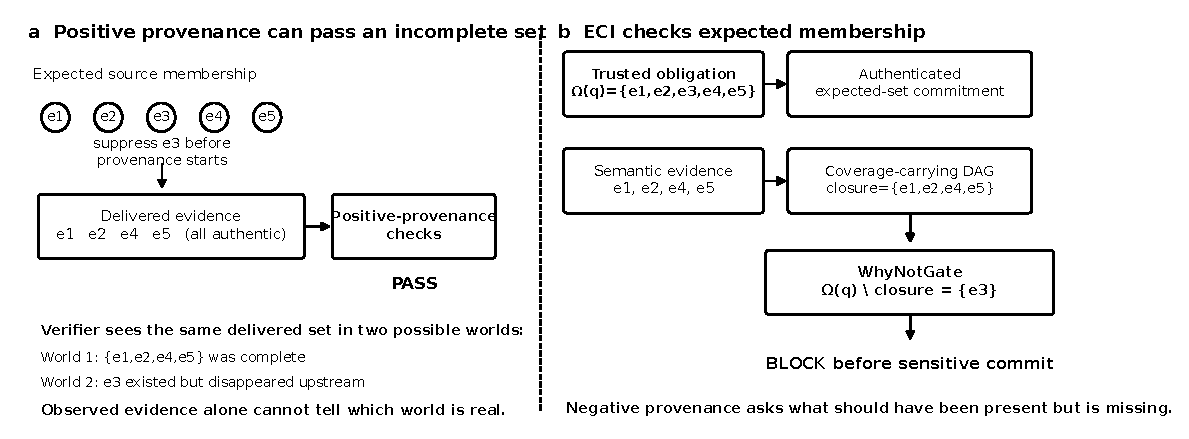
\includegraphics[width=0.98\textwidth]{fig1_omissionshield_overview.pdf}
  \caption{Positive provenance versus Evidence Completeness Integrity. Left: all delivered items can be authentic and provenance-valid even when a required source member was suppressed before the trace began; the delivered trace alone cannot distinguish a genuinely complete set from a silently reduced one. Right: \system{} commits to the expected source membership independently, propagates transitive source coverage, and blocks the sensitive commit when $\Omega(q)\setminus(\mathrm{Closure}_{src}\cup A_{drop})$ is nonempty.}
  \label{fig:overview}
\end{figure*}

Our contributions are:
\begin{itemize}
  \item We formulate SES as an integrity attack on the membership of a bounded evidence set and introduce \emph{Minimal Decisive Omission} (MDO) as the smallest tested suppression budget that reaches an attacker-preferred decision.
  \item We formalize ECI and prove an observation-equivalence boundary: a verifier that sees only delivered evidence plus metadata derived from that evidence cannot distinguish a genuinely complete small set from a larger set that was silently reduced upstream.
  \item We present \system{} as a compositional reference-monitor design for ECI, with an authenticated source obligation, runtime-owned coverage representation, authenticated drop authorizations, and WhyNotGate. A flat authenticated source-ID certificate is an equivalent simpler representation when the complete coverage set can be carried unchanged to the sink.
  \item We evaluate SES primarily on 49 public multi-file security-fixing commits with frozen intervention protocols and an independent 7B replication. We use a separately frozen 200-alert SecAlertBench cohort as a secondary cross-domain stress test to expose evidence-type and operating-point dependence rather than to estimate production SOC fragility.
  \item We evaluate the trusted runtime beyond a single hop: 3,328 genuine real-domain single-item evidence removals are rejected with exact missing-ID attribution; 419 additional SOC schema-item checks cover already-absent field placeholders and are disclosed separately. Multi-stage compression preserves transitive source accountability through up to five aggregation layers, and we report measured control-plane latency and footprint. We explicitly separate structural completeness---which we enforce---from semantic faithfulness, which we do not claim.
\end{itemize}

\section{Related Work}
\subsection{Information-flow and Authenticated Execution}
Fides formalizes security/expressiveness trade-offs for agent planners and uses dynamic integrity/confidentiality labels with deterministic policy enforcement~\cite{costa2025fides}. Authenticated Workflows binds prompt, tool, data, and context boundaries cryptographically~\cite{rajagopalan2026authenticated}, while CXI focuses authority checks at protected execution sinks~\cite{santos2026cxi}. These systems protect important properties of values and actions that participate in an execution. ECI addresses a different input to the security decision: an independently expected source membership set. Our code audit of the public Fides Gateway found that its ``total coverage'' check refers to resolvable IFC labels on queryable JSON roots/paths, not to completeness of an external bounded source result set.

\subsection{Evidence Tracing, Runtime Provenance Gates, and Task Contracts}
Agent provenance work connects retrieved evidence, intermediate claims, memory, tools, and outputs~\cite{wang2026traces}. Very recent systems increasingly connect provenance to trusted intent and realized effects. AGATE places deterministic authorization and data-provenance checks at instrumented agent-harness boundaries; its public abstract states that source registration connects \emph{observed inputs} to later transfers and identifies observation coverage as a concrete limit~\cite{zhang2026agate}. Matrix records deterministic causal state for authority, facts, and completion evidence, and reports that an authored completeness contract can over-block when transferred outside its authoring context~\cite{salas2026governed}. TraceGrant establishes a task-effect Contract from the trusted user request, constrains admitted evidence to authority already established by that Contract, and verifies completion against actual tool results~\cite{tracegrant2026}. These mechanisms substantially overlap with \system{} at runtime enforcement, provenance, and contract checking, so those layers are not claimed as novel in isolation. The narrower distinction is the protected object and reference information available before the trace: ECI commits to an independently enumerated \emph{source-membership set} and checks whether each required member remains transitively covered at commit. The public descriptions we verified do not state the same delivered-only observation-equivalence result or describe an authenticated expected source-member set whose missing members are carried as negative provenance through transformed evidence. This statement is intentionally limited to the verified public descriptions, not to unverified implementation details. AID-Guard separately closes authorization over provider state, retries, and recovery~\cite{aidguard2026}. AgentDojo provides a complementary benchmark for prompt-injection attacks on tool-using agents~\cite{debenedetti2024agentdojo}; SES instead removes evidence without injecting instructions.

\subsection{Adversarial Missingness and Robust Decision-Making}
Koyuncu et al. introduced adversarial missingness as a training-data attack that deceptively omits authentic samples to bias causal-structure learning, including settings where observed samples can be cryptographically audited~\cite{koyuncu2023missingness}; a 2024 TIST extension develops that attack class further~\cite{koyuncu2024tist}. Their AAAI-26 follow-up broadens adversarial missingness to common remediation procedures such as complete-case analysis and imputation and explicitly notes the lack of defense strategies for that threat class~\cite{koyuncu2026remediation}. These works are the closest conceptual precedent for ``truthful data made unavailable by an adversary.'' SES differs in attack surface and security object: it targets runtime membership of a task-bounded evidence set immediately upstream of a decision, while ECI introduces an authenticated expected-set obligation and fail-closed commit-time structural enforcement. More broadly, robust Bayesian decision work studies decisions and data acquisition under adversarial uncertainty in outcome variables~\cite{harikumar2026robust}. Earlier evidence-theoretic work, including our prior NECM study combining neutrosophic representations with belief-function reasoning for ambiguity and rejection, addressed uncertainty within the evidence that is available~\cite{guo2015necm}; SES instead asks whether the availability of otherwise truthful evidence is itself adversarially controlled. We therefore use MDO only as a concrete intervention metric for the present experiments rather than introducing an unused general decision-theoretic layer.

\subsection{Omission and Missing Answers}
Rajan et al. show that omission can arise throughout an agent pipeline, including deterministic ingestion/protocol layers and behavioral model layers, and quantify the phenomenon across controlled and real-agent pilots~\cite{rajan2026missing}. Their work substantially motivates the problem but treats omission primarily as a reliability/attribution phenomenon. Kemeklis and Vemuri define omission attacks in AI control where the adversary fails to perform a necessary action and propose postcondition monitoring in an AI Control Hackathon 2026 sprint project~\cite{kemeklis2026omission}. We therefore avoid using ``omission attack'' as our threat name: SES concerns removal of evidence, not omission of an action. Chen et al. independently show that LLM-authored sets are vulnerable to silent omissions and that missing members are harder to audit than present errors~\cite{chen2026enumerating}. Database why-not provenance provides the deeper conceptual precedent for explaining absent query answers~\cite{lee2017whynot,lee2018pug}. Our contribution is not the invention of why-not provenance; it is a security contract that carries an expected bounded source set through an agent evidence DAG and enforces its coverage at decision commit.


\begin{table*}[t]
\centering
\caption{Closest-neighbor comparison. Entries describe only features verified from the cited public descriptions; ``not established'' is not a claim about unverified implementation details.}
\label{tab:neighbors}
\small
\resizebox{\textwidth}{!}{%
\begin{tabular}{p{0.14\textwidth}p{0.24\textwidth}p{0.20\textwidth}p{0.20\textwidth}p{0.14\textwidth}}
\toprule
Work & Primary protected object & Evidence reference point & Expected source-member absence property & Commit-time enforcement \\
\midrule
AGATE~\cite{zhang2026agate} & Authorization + provenance of data carried into effects & Registered observed sources & Not established in verified abstract & Yes \\
Matrix~\cite{salas2026governed} & Governed authority, facts, completion & Authored contracts + causal state & Completeness contract, but source-member absence not established & Yes \\
TraceGrant~\cite{tracegrant2026} & Trusted task intent through realized effects/completion & Contract + admitted runtime evidence & Independent expected source-member set not established & Yes \\
\system{} & Bounded expected source membership & Authenticated external expected set + runtime coverage & Yes: ECI & Yes \\
\bottomrule
\end{tabular}%
}
\end{table*}

\section{Threat Model and Problem Formulation}
\subsection{Bounded Evidence Tasks}
A task $q$ reads from a source for which a trusted component can enumerate, or cryptographically commit to, a finite task-required universe $\Omega(q)=\{e_1,\ldots,e_n\}$. Examples include the files changed between two Git commits, rows matching a database predicate, alerts in a fixed incident window, records enumerated by a paginated API that exposes a trusted total/continuation structure, or a workflow in which a fixed set of upstream agents is required to report.

The decision procedure may be an LLM, deterministic program, or hybrid system. We denote the final decision by $D(E)$ for the evidence delivered to the decision point. ECI is not a correctness specification for $D$; it constrains whether $D$ is allowed to commit using a structurally incomplete required set.

\subsection{Selective Evidence Suppression}
The SES adversary acts on \emph{structural membership}: it may drop, truncate, selectively forward, or suppress required evidence between source enumeration and the decision point. A concrete deployment example is a compromised or faulty pagination/retrieval-merger service that can omit returned records or continuation pages but cannot forge the independently authenticated source commitment or modify payloads that do arrive. It may choose which members to suppress adaptively based on the desired outcome and may control a deterministic pagination/transport/cache layer, retrieval merger, context assembler, deterministic routing or truncation layer, or orchestration component that can remove evidence handles. Adaptivity therefore refers to the choice of the suppression set $S$, not to arbitrary semantic corruption of evidence that has already been delivered. Our exhaustive subset search in the evaluation is an attack-surface oracle: it establishes whether a small decisive suppression exists, not that every attacker can discover the optimum with the same query cost. A weaker attacker with limited model access can realize only a subset of these suppressions; the ECI guarantee itself is independent of how the attacker selects the omitted items.

The attacker may \emph{not} alter the trusted task obligation, forge a source commitment or evidence identity, modify the values of evidence that remains visible, or mint trusted provenance edges. Semantic mischaracterization after structural delivery is a distinct threat class outside the ECI property and is treated separately below. Our primary attack deliberately avoids explicit malicious instructions. Thus, after suppression, all observed evidence may continue to pass content, signature, provenance, and information-flow checks designed for observed objects.

For target outcome $a\neq D(E^\star)$, define
\begin{equation}
  \mathrm{MDO}(E^\star,a)=\min_{S\subseteq E^\star}|S|
  \quad\mathrm{s.t.}\quad D(E^\star\setminus S)=a,
\end{equation}
with MDO undefined (or $\infty$) if the target outcome is unreachable under the tested suppression family. In our experiments, $D$ denotes the fixed deterministic evaluation protocol (fixed model configuration, decoding rule, and seed where applicable), and we report MDO only over subsets that were actually evaluated. A low MDO therefore denotes a small tested structural attack surface; it is not a population-level risk estimate.

\subsection{Control-plane Coverage Instead of Full Raw Forwarding}
A naive response to suppression is to forward every raw source object to the final model. ECI does not require that. The semantic data plane may carry summaries or other compact derived artifacts, while the trusted control plane carries source identifiers and ancestry sufficient to establish structural coverage. Thus the final verifier need not receive every raw payload. When a complete authenticated source-ID set can simply be carried unchanged to the sink, a flat manifest is sufficient and the DAG is unnecessary; the DAG is useful only when the workflow needs localized ancestry or incremental composition across transformed artifacts. We do not claim semantic sufficiency or semantic faithfulness of such transformations in this paper.

\begin{table*}[t]
\centering
\caption{Five mechanism classes and the absence information available at commit. A check mark means the mechanism can establish the property under the stated special-case assumptions; ``observed only'' means it reasons from evidence already admitted to the trace.}
\label{tab:five-class}
\small
\resizebox{\textwidth}{!}{%
\begin{tabular}{p{0.20\textwidth}p{0.20\textwidth}p{0.17\textwidth}p{0.18\textwidth}p{0.17\textwidth}}
\toprule
Mechanism class & Commit-time reference & Pre-trace missing member? & Through transformed evidence? & Deterministic commit check? \\
\midrule
Fixed-schema validation & Fixed required fields & Yes, for that fixed schema & No, unless schema state is forwarded & Yes \\
Direct authenticated manifest & Expected source-ID set + forwarded IDs & Yes & Only if full coverage set is forwarded & Yes \\
Positive provenance / tracing & Observed/admitted evidence & No & Yes for observed ancestry & Usually not completeness \\
Runtime provenance / task-effect gates & Registered evidence + authority/effect contract & Observed only in verified descriptions & Yes & Yes \\
ECI / \system{} & Authenticated expected source-membership set & Yes & Yes, via transitive source coverage & Yes \\
\bottomrule
\end{tabular}%
}
\end{table*}

\subsection{Trust Boundary and Non-goals}
\begin{table*}[t]
\centering
\caption{Trusted computing base and adversary boundary.}
\label{tab:tcb}
\small
\begin{tabular}{p{0.25\textwidth}p{0.12\textwidth}p{0.54\textwidth}}
\toprule
Component & Status & Role \\
\midrule
Task specification $q$ & Trusted input & Defines the bounded query/task whose required source membership is to be protected; if attacker-controlled or underspecified, ECI cannot repair a wrongly scoped obligation. \\
Bounded source / obligation compiler & Trusted & Given trusted $q$, enumerates or commits to the task-relevant required source-ID universe. \\
Runtime transfer instrumentation & Trusted & Records handles that actually cross stage boundaries; models cannot mint parent edges. \\
Approved-drop authority & Trusted & Authenticates any waiver that removes a required source ID from the commit-time obligation. \\
LLM / agent / ordinary orchestrator & Untrusted & May omit, truncate, or selectively forward evidence; arbitrary semantic output remains untrusted but is outside the ECI completeness guarantee. \\
WhyNotGate / commitment verifier & Trusted & Checks the authenticated obligation, approved drops, and terminal source closure before sensitive commit. \\
\bottomrule
\end{tabular}
\end{table*}

The LLM, intermediate agent logic, and ordinary orchestration are outside the trusted computing base. If the same compromised component both chooses the evidence and declares that the chosen set was complete, the observation-equivalence boundary applies immediately. The bounded source/obligation compiler, runtime transfer instrumentation, and final gate are trusted in the present design. This is a \emph{localization} of trust, not an elimination of trust: ECI moves completeness authority out of the broad, model-facing orchestration path and into a narrow expected-set boundary plus reference-monitor design. Proposition~1 shows this necessity only for verifiers whose inputs are restricted to delivered evidence and metadata derived solely from it; a verifier that receives an independent authenticated expected-set signal is outside the proposition's premise. \system{} does not solve compromise of the authority that defines that set. If $\Omega(q)$ is itself generated or scoped by an LLM, ECI inherits omissions made by that LLM in obligation construction; the downstream gate cannot repair a wrongly scoped expected set.

We do not claim open-world completeness. If a web search returns ten documents, the system cannot infer from those ten alone that an eleventh relevant document does not exist. We also do not claim semantic preservation through arbitrary LLM transformations. A derived summary may structurally cite every required parent yet semantically misrepresent one; that problem requires a distinct semantic-faithfulness mechanism. Finally, ECI complements rather than replaces source authenticity, IFC, tool authorization, prompt-injection defenses, or claim grounding.

\section{Why Positive Evidence Is Insufficient}
Existing controls commonly validate properties of evidence that is present: signatures, integrity labels, source ancestry, causal support, or evidence-handle membership. Such checks are valuable but face an information boundary when expected-set information is absent.

\begin{proposition}[Observation-equivalence necessity]
Let verifier $V$ receive an observation $(E,M)$, where $E$ is a finite delivered evidence set and $M$ is auxiliary metadata generated solely from $E$ (deterministically, $M=f(E)$; or randomly, according to a distribution conditioned only on $E$). Then there exist two worlds---one in which $E$ is the complete required universe and one in which the required universe is $E\cup\{x\}$ for some $x\notin E$ but $x$ is suppressed before observation---that induce the same observation distribution for $V$. Consequently, $V$ has the same output distribution in the two worlds and cannot distinguish expected-set completeness from pre-observation suppression under this input condition.
\end{proposition}
\begin{proof}
Consider $W_0$, where the complete required universe is exactly $E$, and $W_1$, where the required universe is $E\cup\{x\}$ but $x$ is removed before any input visible to $V$ is generated. The delivered set is $E$ in both worlds. By the proposition's premise, $M$ is generated only from $E$, so its conditional distribution is also identical in $W_0$ and $W_1$. Hence the joint observation $(E,M)$ has the same distribution in both worlds. Any deterministic verifier therefore returns the same output, and any randomized verifier has the same output distribution.
\end{proof}

The premise is deliberately syntactic: $V$ sees only the delivered set and quantities generated from that delivered set. The proposition therefore does \emph{not} apply to a verifier that already receives trusted information about the expected universe. For example, an authenticated total count, trusted sequence/continuation structure, signed source manifest, or Merkle commitment is not a function solely of the delivered $E$ when it encodes information about members that may be absent. Such mechanisms are precisely ways to escape the observation-equivalence condition. The result does not imply that positive provenance or IFC is weak at its intended property; it identifies the input condition under which expected-set completeness is information-theoretically unavailable. Database research has long distinguished why-provenance from why-not explanations for missing answers~\cite{lee2017whynot,lee2018pug}; \system{} adapts this negative-provenance perspective to source-to-decision security in LLM-agent pipelines.

\section{OmissionShield Design}
\subsection{Control Plane vs. Semantic Data Plane}
A central design choice is to avoid hashing or otherwise constraining free-form natural language. The semantic data plane remains unconstrained: an agent may summarize, rank, compare, or rewrite evidence. Separately, the evidence control plane represents immutable source evidence by stable handles and represents every accepted derived artifact by explicit parent handles.

Each source node has identifier $e_i$ and payload digest. Each derived node $v$ contains a set $\mathrm{Parents}(v)$ of evidence handles. For terminal artifacts $T$ used to support a sensitive decision, the control plane computes $\mathrm{Closure}_{src}(T)$, the set of source nodes reachable by recursively following parent edges.

This separation addresses an important systems mismatch. Cryptographic hashes are meaningful for source objects and control-plane commitments, but a natural-language summary is not byte-identical to its source. \system{} therefore never claims that a summary hash proves semantic preservation. It proves only which source objects were structurally accounted for in the transformation graph.

\subsection{Evidence Obligations and Source Commitments}
For each bounded task, a trusted task specification $q$ fixes the query/scope whose evidence membership is security-relevant, and a trusted source/obligation component constructs $\Omega(q)$ and a commitment $R_q=\mathrm{Commit}(\Omega(q))$. Our prototype hashes a canonicalized ID set; the commitment binds source IDs rather than payload bytes or source versions. Payload integrity is delegated to the authenticated source layer, and IDs are assumed unique within a task instance. A deployment could instead use signed manifests, Merkle structures, authenticated pagination metadata, or source-specific commitments and should bind an epoch/version for dynamic sources.

The trusted computing base must include both the correctness of the task specification and the task-relevance judgment encoded by this enumeration. This is unavoidable: if the component defining the expected universe itself omits $x$, no downstream verifier can recover that fact from absence alone, by Proposition~1.

\subsection{Coverage-Carrying Evidence DAG}
Every cross-agent or cross-stage transformation produces both a semantic artifact and a control-plane evidence node. A coordinator that summarizes 100 alerts may output a short paragraph on the data plane and a derived handle whose parent set names the relevant input handles on the control plane. A later synthesis artifact can cite that summary handle, preserving transitive source ancestry without repeatedly embedding the raw records into the model context.

Evidence loss is either structurally visible as the absence of a required source from the terminal closure or explicitly represented by a \emph{drop record}. Drop records support policy-approved transformations such as privacy minimization. The security distinction is therefore not ``nothing may ever be removed'' but ``required removal may not be silent.''

\subsection{Evidence Completeness Integrity and WhyNotGate}
\begin{definition}[Evidence Completeness Integrity]
For a bounded task $q$ with authenticated required-source set $\Omega(q)$, terminal artifacts $T$, and authenticated task-bound approved drops $A_{drop}$, structural Evidence Completeness Integrity (ECI) holds at a protected commit iff
\[
\Omega(q)\subseteq \mathrm{Closure}_{src}(T)\cup A_{drop}.
\]
ECI is a structural membership property only: it does not imply that a derived natural-language artifact semantically used, faithfully summarized, or correctly interpreted every covered source item.
\end{definition}

Immediately before a sensitive decision commits, WhyNotGate receives the task obligation, source commitment, terminal evidence handles, and approved-drop records. It rejects on source-commitment mismatch or whenever
\begin{equation}
 \Omega(q)\setminus\left(\mathrm{Closure}_{src}(T)\cup A_{drop}\right)\neq\emptyset.
\end{equation}
The gate is fail closed. On success it may release the proposed decision to the sensitive sink; on failure it returns a secure abstention carrying the exact missing evidence IDs, and no protected side effect is committed. The orchestrator may then retrieve the missing evidence, obtain an authorized drop, or terminate the task, but any later decision must pass a fresh gate check. Thus detection and enforcement are coupled at the commit boundary rather than left to model discretion.

\begin{theorem}[Post-obligation structural completeness safety]
Fix a trusted task specification $q$ and terminal decision artifacts $T$. Assume: (i) before attacker-controlled downstream processing, a trusted obligation authority correctly constructs the task-relevant $\Omega(q)$ implied by $q$ and authenticates a commitment to it; (ii) source identities, that commitment, and approved-drop authorizations are unforgeable to the attacker; (iii) trusted runtime instrumentation creates a derived-node parent edge only from an evidence handle actually delivered across the corresponding stage boundary; (iv) WhyNotGate faithfully verifies the commitment and admits only if
\[
\Omega(q)\setminus\bigl(\mathrm{Closure}_{src}(T)\cup A_{drop}\bigr)=\emptyset,
\]
where $A_{drop}$ contains only authenticated, task-bound approved drops; and (v) every protected security-sensitive sink is completely mediated by WhyNotGate, so attacker-controlled orchestration cannot release the protected effect through an ungated path. Then for every required source item $x\in\Omega(q)\setminus A_{drop}$, if attacker-controlled processing removes all runtime-recorded paths from $x$ to $T$, WhyNotGate rejects the decision commit.
\end{theorem}
\begin{proof}
Take any $x\in\Omega(q)\setminus A_{drop}$ whose runtime-recorded paths to $T$ have all been removed. By assumption (iii), later untrusted stages cannot recreate coverage of $x$ merely by naming it: a parent edge can arise only from a handle that was actually delivered. Hence $x\notin\mathrm{Closure}_{src}(T)$. Because $x\notin A_{drop}$ as well, $x$ remains in the set difference checked by assumption (iv), which is therefore nonempty, so WhyNotGate rejects. Acceptance is possible only if a real structural path to $x$ is restored, an authenticated drop for $x$ is supplied, or one of the stated trust assumptions fails.
\end{proof}

The theorem is deliberately conditional and soundness-only: it proves that an accepted protected commit cannot silently lose a required structural obligation under assumptions (i)--(v); it does not by itself prove availability or that every complete benign execution will be admitted. Complete-trace admission is evaluated empirically below. The current Python prototype also does not instantiate assumption (iii) against arbitrary same-process compromise: \texttt{deliver()} and \texttt{enumerate\_source()} are public methods, the HMAC key resides in-process, and the stdio setup creates the runtime in the same process as untrusted context construction. Audit probes can therefore forge apparent delivery if they already control that process. The theorem treats runtime transfer instrumentation and complete mediation as trusted deployment assumptions, not properties proved by the in-process prototype.

The theorem is deliberately conditional. It does not establish that the obligation authority chose the correct universe; Proposition~1 shows why that upstream fact cannot be reconstructed from downstream positive evidence alone. Its guarantee begins \emph{after} a correct expected-set commitment and prevents silent loss within the instrumented downstream path. Proposition~1 and Theorem~1 therefore separate two questions that should not be conflated: an independent expected-set signal is necessary to define completeness for a delivered-only verifier, while ECI is sufficient to enforce that defined structural obligation against downstream suppression under the stated TCB and complete-mediation assumption.

\noindent\textbf{Composition consequence.}
Under Theorem~1's assumptions, if a required source item $x\in\Omega(q)\setminus A_{drop}$ has no runtime-recorded path to the current frontier, then adding further correctly instrumented layers cannot place $x$ in a later terminal source closure unless a later stage actually reintroduces a handle with a valid path to $x$. This is a direct consequence of transitive reachability rather than an independent theorem: later derived nodes inherit only the source coverage of runtime-recorded parents. Redundant paths are allowed, so suppressing one branch is harmless when another ancestry still covers the same required source ID.

\section{Security Analysis Beyond the Core Theorem}
The theorem isolates one enforceable property, but a deployment exposes several adjacent attack surfaces. We therefore distinguish attacks that ECI closes from attacks that require another mechanism.

\noindent\textbf{Suppression after trusted enumeration.}
This is the intended SES case. Once a correct obligation is authenticated, dropping a required source object or any derived branch whose transitive closure contains required sources makes those source IDs absent from the terminal closure. WhyNotGate therefore rejects independently of the model's natural-language behavior.

\noindent\textbf{Compromised obligation construction.}
If the source or obligation compiler omits an item before commitment, downstream ECI cannot infer that the omitted object should have existed. This is not an implementation accident; it follows directly from observation equivalence. Deployment must therefore place source enumeration inside the trusted computing base or obtain the expected set from an independently authenticated mechanism such as a signed manifest, Merkleized query result, or trusted pagination protocol.

\noindent\textbf{Forged ancestry and model self-report.}
A compromised model may state that it used an evidence item it never received. Such text is not a trusted edge. In \system, parent relations are produced only from runtime-observed handle delivery. An adversary that can forge those runtime records has crossed the stated TCB boundary; an adversary confined to model output or ordinary orchestration cannot repair a missing structural path by assertion.

\noindent\textbf{Semantic suppression after structural delivery.}
A stage may receive every required handle yet semantically ignore, downweight, or mischaracterize one source in its summary. ECI can accept such a trace because structural delivery occurred. This is not an adaptive SES action under our threat definition: SES adaptivity is over which membership elements to remove, whereas semantic rewriting after delivery is a separate corruption capability outside the ECI property. Consequently, the empirical deletion attacks measure the security consequence of \emph{membership suppression}, not the prevalence or severity of semantic manipulation. Semantic-faithfulness verification, claim-level grounding, or redundant review can be composed above ECI, but they solve a different problem and are not evaluated here. The narrower claim remains useful because structural omission can occur in deterministic pagination, transport, caching, routing, truncation, retrieval merging, or context assembly before any semantic reasoning takes place. An adversary with arbitrary semantic-rewrite control over an LLM summarizer is strictly stronger than the SES adversary studied here and is outside the ECI guarantee.

\noindent\textbf{Approved-drop abuse.}
Policy-approved drops intentionally waive structural coverage for named evidence IDs, for example to support minimization. The authority that issues such waivers is therefore security-sensitive. The prototype now implements a minimal authenticated drop token that binds the task ID, evidence ID, source root, policy principal, reason, and nonce under a drop-authority key; forged signatures, wrong-task tokens, stale source-version tokens, and nonce replay are rejected in regression tests. This mechanism authenticates a waiver after a policy authority has decided to issue it; it is not a full policy-decision service. All primary Git, SOC, composition, and mechanism-ablation enforcement results use $A_{drop}=\emptyset$; approved drops are exercised only in dedicated authorization tests.

\noindent\textbf{Replay and stale obligations.}
The obligation HMAC binds task ID, required IDs, and source root. Drop tokens additionally bind the source root and a one-use nonce, so a waiver issued for one task/source version cannot be replayed against a different obligation in the reference runtime. A production protocol should still bind a stronger freshness epoch or source version when task identifiers themselves can be replayed across runtime restarts.

\noindent\textbf{Content modification.}
SES deliberately assumes that delivered evidence values remain authentic. If an attacker can modify payloads, source authenticity or IFC must protect those values. ECI complements these mechanisms by checking membership; it is not a replacement for them.

This attack-surface decomposition matters because it prevents an unrealistically broad claim. \system{} converts a specific class of invisible membership manipulation into a deterministic policy failure, while leaving source compromise, semantic misrepresentation, and content tampering to explicitly separate controls.

\section{Implementation}
The reference prototype is implemented in Python and deliberately keeps the trusted mechanism small. Its trusted control plane consists of source enumeration, authenticated evidence obligations, runtime-owned delivery records, evidence-node construction, authenticated drop-token verification, and WhyNotGate. The evidence DAG stores source and derived nodes, immutable IDs, parent relations, and explicit drop records. Obligations store a required-source-ID set and a deterministic source commitment. Drop authorizations are HMAC-bound to task ID, evidence ID, source root, policy principal, reason, and a one-use nonce; the implementation optionally uses a key distinct from the source-obligation key.

A key design rule is that the LLM and untrusted orchestrator do \emph{not} self-report provenance edges. The \texttt{TrustedEvidenceRuntime} records the handles that actually cross each instrumented stage boundary. When a stage emits a derived artifact, the runtime assigns its structural parents from the previously recorded delivery event rather than from model-generated text. In the prototype, the obligation is HMAC-bound to the task identifier, canonicalized required-ID set, and source root. Consequently, a model may claim in natural language that it consumed an omitted record, but that statement cannot create the missing control-plane edge. This mechanism proves structural transfer, not semantic use. The in-process Python object is a functional implementation of the reference-monitor logic, not a proof of privilege isolation against arbitrary same-process code execution; Theorem~1 treats transfer instrumentation and complete mediation as trusted. A production deployment must place that instrumentation and the commit gate behind a mediation boundary that untrusted orchestration cannot bypass.

We implemented a Git adapter as a concrete bounded source. The expected universe is obtained independently from \texttt{git diff --name-only BASE HEAD}; each changed path becomes a source evidence ID. A complete review context passes. If an intermediate stage suppresses one changed path, the downstream source closure lacks that path and WhyNotGate reports it exactly. We also implemented a three-stage collector--reviewer--commit prototype. In the attack configuration, \texttt{auth.py} is suppressed before review and the unprotected workflow commits a benign judgment; under ECI, the same workflow is blocked at commit with \texttt{auth.py} reported as the missing obligation member.

To exercise an actual tool-protocol boundary rather than only in-process function calls, we additionally built a minimal JSON-RPC 2.0 stdio integration using a separate child-process tool server. The experiment executes the protocol methods \texttt{initialize}, \texttt{tools/list}, and \texttt{tools/call}; a source tool returns structured evidence items, untrusted context construction may suppress one returned item, and a gateway in the agent-side process runs WhyNotGate immediately before a security-sensitive decision tool in the child process is invoked. The integration intentionally does not claim conformance with a particular MCP SDK implementation or OS-enforced privilege separation. Instead, it demonstrates gating of a concrete cross-process tool call, not a cross-process isolated gate: the gateway/runtime remains agent-side in the prototype; production security still requires that this mediation path cannot be bypassed by the orchestrator.

The codebase includes regression tests for observation equivalence, commitment mismatch, structurally complete summaries, silent parent omission, authenticated approved drops, forged/wrong-task/stale/replayed drop tokens, semantic-faithfulness non-guarantees, forged obligations, model attempts to self-report parents, Git-backed set enumeration, multi-layer composition, and the stdio tool boundary. At the current revision, all 29 project tests pass.

\section{Evaluation}
We evaluate eleven questions: (1) can selective suppression alter decisions on independently sourced security patches; (2) does the effect reproduce in a frozen holdout cohort; (3) how small are successful suppressions; (4) does the effect persist across model families; (5) does SES replicate in a distinct production-derived SOC-triage domain; (6) how does selective deletion compare with random loss at the same budget; (7) does ECI detect structural suppression while admitting complete executions in both domains; (8) does coverage compose through multiple aggregation layers; (9) how do positive provenance, terminal-only checks, a flat full-forward coverage certificate, and DAG-based ECI differ as enforcement representations; (10) can the gate mediate a real cross-process tool-call boundary rather than only an in-process harness; and (11) what overhead and metadata footprint does the reference mechanism add?

\subsection{Public Security-Patch Cohorts}
We used the TQRG ground-truth security-patch dataset, which aggregates thousands of public security-relevant commits across many projects and vulnerability classes~\cite{reis2021tqrg}. To avoid selecting examples after observing model behavior, cohort construction used metadata only. We required a CVE identifier, a GitHub project and valid commit SHA, two to five changed files, 4--180 changed lines in the dataset metadata, at least one source-code-like extension, and unique project and CVE membership. A fixed seed determined the ordering.

The first 20 candidates were frozen before GitHub patch retrieval. Nineteen were retrievable; one returned an HTTP 422 response and was excluded under the pre-specified ``commit inaccessible'' rule. We then froze the next 30 metadata-selected candidates as a holdout cohort before retrieving any of their patches or observing any holdout model outputs; all 30 were retrievable. Thus the analysis contains 49 public multi-file security-fixing commits from distinct project/CVE selections. Two commits included binary fixture files for which GitHub exposed no textual patch; those files remained in the structural ECI obligation, but the LLM received only the available textual patches.

For each commit, the model saw only per-file patch text: no CVE identifier, vulnerability label, commit message, or TQRG security metadata. The primary run called the localhost Ollama server at \texttt{127.0.0.1:11434} through the hard-coded endpoint in \texttt{src/phase0c\_llm.py}; the frozen trial logs record the mutable tag \texttt{qwen3:latest}, temperature zero, and \texttt{/no\_think}, but not an immutable model digest. A live host check after the experiments shows that \texttt{qwen3:latest} resolves on this machine to architecture qwen3, 8.2B parameters, Q4\_K\_M quantization, context length 40960, with model-layer digest \texttt{sha256:a3de86cd\allowbreak{}1c132c82\allowbreak{}2487eded\allowbreak{}d47a324c\allowbreak{}50491393\allowbreak{}e6565cd1\allowbreak{}4bafa40d\allowbreak{}0b8e686f}. The corresponding manifest and 5,225,374,496-byte model blob both have filesystem modification times of March 10, 2026, predating the August--September 2026 experiments and indicating that this host image had been present unmodified since before the runs. Thus the host record supports the qwen3 8.2B Q4\_K\_M identity linkage, but the exact historical digest is still not logged in the trial artifacts themselves. We used deterministic decoding with temperature zero, seed 20260824, and the \texttt{/no\_think} instruction; it classified the complete patch set as \texttt{SECURITY\_FIX} or \texttt{NO\_SECURITY\_FIX}. We define a model--commit case as \emph{competent} only when the model recognized the known security-fixing commit under complete evidence. This conditioning prevents base-model inability to recognize a vulnerability fix from being mislabeled as suppression robustness. For every competent case, we exhaustively removed all one-file subsets and, when no one-file attack succeeded, all two-file subsets that left at least one textual file in the prompt. The empirical MDO is the smallest tested removal set that changes the judgment to \texttt{NO\_SECURITY\_FIX}.

\subsection{Second Domain: Production-derived SOC Alerts}
As a secondary cross-domain stress test, we added SecAlertBench, a public Tier-1 SOC-triage artifact constructed from alerts collected in the production SOC environments of three large enterprises~\cite{secalertbench2026}. The released processed dataset contains 8,322 normalized alerts spanning 241 distinct \texttt{rule\_name} values (and 23 distinct \texttt{attack\_type} values): 2,496 labeled \texttt{Attack} and 5,826 labeled \texttt{Non-Attack}. The complete raw enterprise logs are not public; our experiment uses only the privacy-processed released artifact. The local dataset is byte-identical to upstream commit \texttt{42a84889\allowbreak fda912ca\allowbreak{}432c9949\allowbreak{}24a1ccd4\allowbreak b9df6274} and has SHA-256 \texttt{33f95305\allowbreak d1c42f8e\allowbreak{}615e4f94\allowbreak{}06611957\allowbreak{}0859dee7\allowbreak eb086dff\allowbreak{}7c227353\allowbreak{}6c932ea3}.

Before any model outputs, we froze a balanced cohort of 100 Attack and 100 Non-Attack records with seed 20260825. Within each label we shuffled deterministically and first maximized distinct alert-rule names before filling the quota; all 100 selected Attack records have distinct rule names. The released schema contains 18 candidate evidence fields after excluding the ground-truth \texttt{Label}, but individual frozen alerts contain only 12--18 nonempty fields (median 16; 16/200 contain all 18). The agent receives the remaining nonempty fields and must output exactly \texttt{ESCALATE} for a real attack or \texttt{CLOSE} for a non-attack. As in the patch benchmark, suppression vulnerability is analyzed only on Attack records the model correctly escalates under complete evidence.

The primary SES intervention exhaustively removes each nonempty field once. We separately froze a stricter \emph{content-only} sensitivity view that excludes \texttt{attack\_type}, \texttt{kill\_chain\_all}, and \texttt{rule\_name} before inference, preventing those taxonomy-like fields from carrying the result by themselves. After observing the pre-specified one-field analysis, and before generating any pair-deletion output, we froze a budget-two follow-up: only complete-evidence-correct Attack records without MDO=1 are eligible, and all unordered pairs of their remaining primary fields are then tested. The alert cohort and evidence definition cannot change in this follow-up.

\subsection{SES Reverses Real Security-Fix Judgments}
In cohort A, Qwen3 recognized 16/19 complete security-fixing patches (84.2\%, Wilson 95\% CI 62.4--94.5\%). Nine of those 16 had MDO=1 and two had MDO=2, yielding 11/16 SES-vulnerable competent commits within budget two (68.8\%, 95\% CI 44.4--85.8\%). Five remained classified as security fixes under every tested one- and two-file removal.

The frozen 30-commit holdout reproduced the effect. Qwen3 recognized 24/30 complete patches (80.0\%, 95\% CI 62.7--90.5\%). Fourteen of those 24 had MDO=1 and one had MDO=2; 15/24 were vulnerable within budget two (62.5\%, 95\% CI 42.7--78.8\%). Nine competent holdout commits did not flip under the tested budget. The holdout therefore did not exhibit an inflated attack rate relative to the first cohort.

Pooled descriptively across both frozen cohorts, 40/49 commits were correctly recognized with complete evidence (81.6\%, 95\% CI 68.6--90.0\%). Of these 40 competent cases, 23 had MDO=1 and three had MDO=2. Thus 26/40 (65.0\%, 95\% CI 49.5--77.9\%) of the full-evidence-correct cases could have their security-fix judgment reversed by suppressing at most two changed-file patches. On the unconditional 49-commit denominator, these are 26/49 (53.1\%) \emph{attack-induced additional misses}: nine commits were already missed with complete evidence, whereas 26 additional commits changed from correct to incorrect only after targeted suppression. Equivalently, allowing the adversary to use zero deletions on already-missed cases and up to two on the others places 35/49 (71.4\%) commits in the attacker-preferred miss state under the tested oracle. The conditional rate measures fragility given baseline competence; the unconditional rate measures added attack impact. Neither is an estimate of production prevalence: the benchmark intentionally selects small, multi-file security-fixing commits to make exhaustive structural intervention feasible.

\subsection{Cross-model Persistence and Competence Boundary}
We repeated the real-commit intervention with Qwen2.5-VL-7B using the same 49 commits and the same evidence-only binary decision task. The run used local weights at \path{/home/yguo56/projects/llm_model/Qwen2.5-VL-7B-Instruct}; the current local \texttt{config.json} has SHA-256 \texttt{77d9ec73\allowbreak{}21cc572e\allowbreak{}3579e2c8\allowbreak{}4799c9ca\allowbreak daded63c\allowbreak{}49ce93b1\allowbreak{}01733349\allowbreak fc330c43}, but the historical cross-model summary did not log the \texttt{--model-path} or Hugging Face revision, so the exact historical checkpoint revision is unrecoverable. The checkpoint was loaded in bfloat16 and decoded greedily (\texttt{do\_sample=False}) with seed 20260824; the 3B control used the same inference path. The Ollama and Transformers protocols were not byte-identical: Qwen3 used \texttt{/no\_think}, slightly more explicit task wording, one request per call, and up to 64 generated tokens, whereas Qwen2.5-VL used the Hugging Face chat template, left-padded batches of two, and up to 10 generated tokens. We therefore interpret this as evidence that omission sensitivity transfers across model/backend configurations, not as a controlled comparison of effect magnitude. The 7B model recognized 44/49 complete patches (89.8\%, Wilson 95\% CI 78.2--95.6\%). Fourteen competent cases had MDO=1 and six additional cases had MDO=2, so 20/44 (45.5\%, 95\% CI 31.7--59.9\%) were vulnerable within two suppressions. On the unconditional denominator, suppression induced 20/49 (40.8\%) additional misses beyond the five complete-evidence misses; under the same zero-to-two-deletion oracle, 25/49 (51.0\%) cases can be placed in the attacker-preferred miss state. The effect is therefore not unique to Qwen3, but its magnitude is model-dependent rather than a universal constant.

We also evaluated Qwen2.5-VL-3B as a lower-capacity control using the corresponding local \texttt{Qwen2.5-VL-3B-Instruct} weights (current local \texttt{config.json} SHA-256 \texttt{7ed3eed5\allowbreak be6924cc\allowbreak{}800e8a5e\allowbreak{}53fc405c\allowbreak{}1aab1aaf\allowbreak{}36bad65c\allowbreak{}33403b36\allowbreak c56827f5}); as with the 7B cross-model run, the historical summary did not log the exact Hugging Face revision, so we do not claim one retroactively. It recognized only 6/49 complete security-fixing commits (12.2\%, 95\% CI 5.7--24.2\%); all six competent cases flipped after a single omission. Because the competence denominator is only six, we do not treat the resulting 100\% conditional flip rate as an estimate of general vulnerability. Instead, the 3B result illustrates why suppression robustness must be conditioned on full-evidence task competence: a model that usually fails before any attack cannot support a meaningful robustness comparison.

\begin{figure}[t]
  \centering
  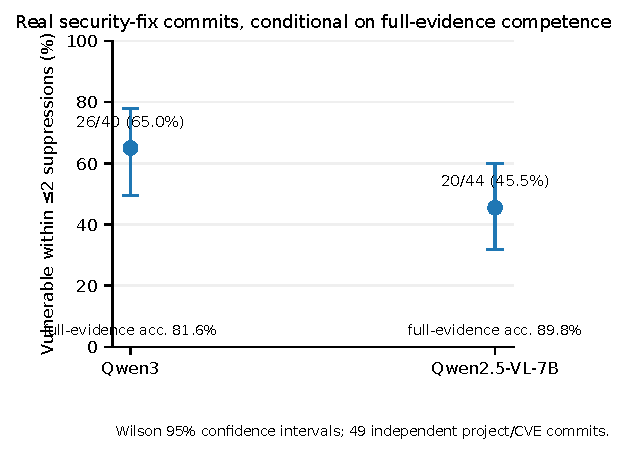
\includegraphics[width=0.98\columnwidth]{fig2_crossmodel_vulnerability.pdf}
  \caption{Cross-model SES vulnerability on the 49 real security-fixing commits. Rates are conditional on correct full-evidence classification; error bars are Wilson 95\% confidence intervals. The 3B model is omitted from the rate comparison because it was competent on only 6/49 complete patches.}
  \label{fig:crossmodel}
\end{figure}

\begin{table}[t]
\centering
\caption{Selective Evidence Suppression on public TQRG security-fixing commits. Vulnerability rates are conditional on correct full-evidence classification.}
\small
\begin{tabular}{lrrrr}
\toprule
Cohort & Full & MDO1 & MDO2 & Vuln. $\leq2$ \\
\midrule
A & 16/19 & 9 & 2 & 11/16 (68.8\%) \\
Frozen B & 24/30 & 14 & 1 & 15/24 (62.5\%) \\
Pooled desc. & 40/49 & 23 & 3 & 26/40 (65.0\%) \\
\bottomrule
\end{tabular}
\end{table}

\subsection{Secondary Cross-domain Stress Test on SOC Triage}
The SecAlertBench intervention provides a qualitatively different security decision: instead of deciding whether a multi-file commit contains a security fix, the agent decides whether a single structured SOC alert should be escalated. We treat this experiment as a stress test of omission sensitivity under a different bounded evidence schema, not as a second headline estimate of deployment-ready model robustness. Qwen2.5-VL-7B correctly escalated 55/100 frozen Attack alerts and correctly closed 46/100 Non-Attack alerts under complete primary evidence, for only 50.5\% balanced-cohort accuracy. Because the operating point is weak, the resulting suppression rates are interpreted only conditionally on complete-evidence correctness and only as evidence that structural deletion can matter in this evidence type.

Among those 55 competent Attack cases, 21 had MDO=1. Of the remaining 34, exhaustive two-field deletion found MDO=2 for another 26. Thus 47/55 (85.5\%, Wilson 95\% CI 73.8--92.4\%) of the full-evidence-correct Attack cases could be changed from \texttt{ESCALATE} to \texttt{CLOSE} by suppressing at most two alert fields. On the unconditional 100-Attack denominator, these are 47/100 (47.0\%) attack-induced additional false negatives beyond the 45 alerts already missed with complete evidence; permitting zero deletions for those baseline misses yields 92/100 Attack alerts in the attacker-preferred \texttt{CLOSE} state under the tested oracle. At each vulnerable alert's case-specific MDO, uniform random deletion hit a target-flipping subset with only 11.0\% mean probability. The effect is not solely attributable to explicit alert taxonomy: 17/21 MDO=1 cases had at least one decisive field outside \texttt{attack\_type}, \texttt{kill\_chain\_all}, and \texttt{rule\_name}. In the separately frozen content-only view that removed those three fields before inference, the model correctly escalated only 23 Attack alerts, but 14/23 (60.9\%, 95\% CI 40.8--77.8\%) of those competent cases still flipped after one additional field suppression. We treat this as a sensitivity analysis because removing the taxonomy fields also changes base-model competence.

Qwen3 exhibited a different operating point on the same primary evidence: it correctly escalated 95/100 Attack alerts but correctly closed only 2/100 Non-Attack alerts, effectively behaving as a highly conservative escalator. Only 4/95 (4.2\%, 95\% CI 1.6--10.3\%) of its correctly escalated Attack cases had MDO=1. We did not run the exhaustive two-field follow-up for Qwen3, so 4.2\% at budget one should not be compared numerically with the 7B model's 85.5\% budget-two rate. The operating-point contrast nevertheless shows an important limitation: SES susceptibility is a property of a model--prompt--decision-rule configuration, not an intrinsic constant of the task. A model that almost never emits \texttt{CLOSE} is harder to drive toward that target by a one-field deletion, but its 98\% false-positive rate would itself make it unsuitable as a standalone triage policy. We therefore report full-evidence behavior next to suppression susceptibility and do not interpret either conditional rate as a deployment prevalence estimate.

ECI enforcement was model-independent in this domain. Treating the 18 released schema positions as the bounded structural obligation, the runtime accepted all 200 complete frozen alert traces and rejected all 3,600 schema-item suppression checks with exact missing-ID attribution. Of these, 3,181 removed fields actually present in the released alert record and 419 removed already-absent field placeholders. Together with 147 genuine Git file removals, the evidence-removal headline is therefore 3,328; the 419 placeholder checks are disclosed separately. This shows that the same expected-set mechanism applies both to variable-size repository manifests and fixed-schema structural obligations, while avoiding the claim that an absent payload is itself removed evidence.

\begin{table}[t]
\centering
\caption{Secondary SecAlertBench stress-test results on the frozen balanced cohort. Full-evidence behavior is shown beside SES rates to prevent conditional omission sensitivity from being read as deployment-ready robustness.}\label{tab:soc-results}
\small
\resizebox{\columnwidth}{!}{%
\begin{tabular}{lrrrr}
\toprule
Model/view & Attack full & Non-Atk full & MDO1 & Vuln. $\leq2$ \\
\midrule
Qwen2.5-VL-7B & 55/100 & 46/100 & 21/55 & 47/55 (85.5\%) \\
7B content-only & 23/100 & 95/100 & 14/23 & -- \\
Qwen3 (Ollama tag) & 95/100 & 2/100 & 4/95 & -- \\
\bottomrule
\end{tabular}%
}
\end{table}

\begin{table}[t]
\centering
\caption{Unconditional attack impact. ``Induced'' counts cases that are correct with complete evidence but enter the attacker-preferred state after suppression. ``Oracle target'' additionally includes cases already in that state at baseline, for which the adversary may choose zero deletions.}
\label{tab:unconditional-impact}
\small
\resizebox{\columnwidth}{!}{%
\begin{tabular}{lrrrr}
\toprule
Setting & Budget & Baseline miss & Induced & Oracle target \\
\midrule
Git, Qwen3 & $\leq2$ & 9/49 (18.4\%) & 26/49 (53.1\%) & 35/49 (71.4\%) \\
Git, Qwen2.5-7B & $\leq2$ & 5/49 (10.2\%) & 20/49 (40.8\%) & 25/49 (51.0\%) \\
SOC Attack, 7B & $\leq2$ & 45/100 (45.0\%) & 47/100 (47.0\%) & 92/100 (92.0\%) \\
SOC Attack, Qwen3 & $\leq1$ & 5/100 (5.0\%) & 4/100 (4.0\%) & 9/100 (9.0\%) \\
\bottomrule
\end{tabular}%
}
\end{table}

Table~\ref{tab:unconditional-impact} separates baseline model error from attack-induced degradation. The conditional MDO rate answers a counterfactual question---among decisions that are correct before the attack, how often can bounded suppression reverse them?---whereas the unconditional induced-error rate answers how much additional error the tested oracle creates on the full cohort. Conditioning therefore does not define which cases are ``near a boundary''; robustly correct cases remain in the denominator and appear as non-vulnerable. Its limitation is instead interpretive: a conditional fragility rate must not be presented as an unconditional deployment prevalence.

\subsection{Selective Suppression Is More Dangerous Than Random Loss}
For each SES-vulnerable real commit, we compared the successful minimal attack with uniform random omission at the same case-specific budget. Because the patch sets contain only two to five files, we can compute the random-hit probability exactly from all size-$k$ combinations rather than simulate it. Among vulnerable cases, the mean probability that random deletion at the MDO budget happened to hit a target-flipping subset was 40.3\% in cohort A and 35.4\% in frozen cohort B (37.5\% pooled descriptively). This is deliberately not a symmetric statistical comparison between two attack algorithms: exhaustive search is an oracle that identifies whether any decisive subset exists, while random deletion measures how often an uninformed loss process would hit one of those subsets at the same budget. Targeted success is therefore one by construction once a decisive subset has been found. The quantity of interest is the size of the gap between existence of a decisive deletion and its measure under uniform deletion, not a claim that a practical attacker obtains the oracle for free.

A separate 60-task controlled suite spans code review, SOC triage, compliance, and procurement with explicit deterministic decision rules. It produced 28 MDO=1, 21 MDO=2, and 11 MDO=3 cases. At each case's MDO budget, uniform random deletion reached the attacker target with 17.2\% mean probability, while an attacker selecting a decisive subset succeeded by construction. We treat this controlled suite as a mechanism stress test rather than real-world evidence.

\subsection{Naturalistic Model Sanity Checks}
Before the public-CVE study, we ran a 20-case hand-authored Qwen3 pilot covering code review and SOC triage. Full-evidence accuracy was 95\%, and deleting one designated decisive item changed 18/20 decisions. We retain this only as a development sanity check. We also created 60 position-controlled variants for Qwen2.5-VL 3B and 7B. The models showed sharply different domain competence, but every variant that was correct under complete evidence changed after the decisive item was removed (28/28 for 3B and 29/29 for 7B). Because those position variants reuse base scenario families, they are repeated measurements and are not pooled with the independent public-CVE cohorts.

\subsection{ECI Functional Validation on Real Commits}
For every public commit, the changed-file manifest supplied the structural evidence obligation independently of the LLM. Across the 49 retrieved commits, the prototype admitted all 49 complete traces. We then suppressed each changed file once, producing 57 single-file structural suppressions in cohort A and 90 in frozen cohort B. WhyNotGate rejected all 147/147 and identified the exact missing path in every case. These deterministic results validate the implementation against the theorem; they are not presented as a statistical contest against learned detectors.

The runtime-owned control-plane tests additionally show why provenance cannot be delegated to model self-report. If a stage receives handles $\{a\}$ but emits text claiming ``I used $a$ and $b$,'' the derived node's parent set remains $\{a\}$ because only the runtime can create transfer edges; a task obligation containing $b$ therefore still fails.

\subsection{Compositional Suppression through Multi-stage Compression}
A journal-length system evaluation should test more than a single collector--reviewer boundary, because real agent pipelines repeatedly compress evidence. We therefore constructed balanced fan-in-four evidence trees with 16, 64, 256, and 1,024 source items, corresponding to 2--5 successive aggregation layers. Each derived node represented the runtime-observed handles delivered to that stage; the final gate saw only the root handle, not the raw source set.

All complete trees were accepted. We then repeated each topology while suppressing one evidence branch at every possible aggregation depth. Across the 14 resulting layer-specific attack conditions, WhyNotGate rejected every execution and recovered the exact underlying source-ID set represented by the missing branch. The number of missing sources grew predictably with attack depth: $[1,4]$ for 16 sources, $[1,4,16]$ for 64, $[1,4,16,64]$ for 256, and $[1,4,16,64,256]$ for 1,024. Thus a high-level omission of one derived summary cannot hide the fact that many original obligations disappeared; transitive source closure converts the missing derived branch back into the corresponding source deficit. Median complete-tree gate time remained 15.6~$\mu$s, 31.9~$\mu$s, 132.7~$\mu$s, and 496.8~$\mu$s at the four sizes, respectively. These are synthetic structural stress tests of composition, not claims about LLM semantic fidelity. Each attack condition suppresses one branch in a balanced fan-in-four tree; we do not claim this experiment covers simultaneous multi-branch suppression, arbitrary fan-in, or cross-task merges.

\subsection{Implementation Tradeoff: Flat Coverage Certificates vs. Compositional Coverage}
This experiment is not intended to show that a coverage DAG is a stronger completeness primitive than an authenticated flat manifest. Instead, it separates the ECI \emph{property} from alternative ways to represent the coverage information needed to enforce it. We reused the balanced fan-in-four trees above and compared four mechanisms while exposing only a single derived root to the sink. A positive-provenance baseline verified that every observed terminal artifact and recorded ancestry edge was locally valid; a terminal-only baseline checked that the sink received exactly one well-formed derived root; ECI expanded the runtime-owned source closure and compared it with the authenticated obligation. As a strong alternative representation, we also evaluated direct source-manifest equality when every original source ID is forwarded unchanged to the final verifier.

Across the four complete trees (16, 64, 256, and 1,024 sources), all four mechanisms accepted. Across the same 14 layer-specific suppression conditions used in the composition experiment, positive provenance and terminal-only checking accepted all 14 reduced executions because the surviving observed structure remained locally valid. Both the full-forward flat manifest and ECI rejected all 14 and recovered the exact missing source set. We therefore do \emph{not} claim a detection advantage for the DAG in this special case: a flat authenticated coverage certificate is security-equivalent when the sink receives the complete source-ID set unchanged. The DAG is our compositional reference representation for workflows in which derived artifacts are chained and the system wants localized ancestry, shared structure, and incremental coverage propagation rather than attaching the full flat coverage set to every derived artifact.

\begin{table}[t]
\centering
\caption{Coverage-representation ablation on transformed multi-stage evidence. The flat-manifest row forwards the complete source-ID coverage set unchanged; ECI represents the same completeness property compositionally through the evidence DAG.}
\label{tab:mechanism-ablation}
\small
\resizebox{\columnwidth}{!}{%
\begin{tabular}{lrrr}
\toprule
Mechanism & Complete accept & Attack reject & Exact missing \\
\midrule
Positive provenance only & 4/4 & 0/14 & -- \\
Terminal-only check & 4/4 & 0/14 & -- \\
Direct manifest (full-forward) & 4/4 & 14/14 & 14/14 \\
ECI transitive coverage & 4/4 & 14/14 & 14/14 \\
\bottomrule
\end{tabular}%
}
\end{table}

\subsection{Cross-process Tool-Boundary Integration}
In the JSON-RPC stdio integration, the source and sensitive-action tools execute in a separate child process. With complete evidence, the protected gateway permits the security decision tool call. When the untrusted context constructor removes \texttt{auth.py}, the same wrong \texttt{NO\_ISSUE} decision reaches the sensitive tool in the unprotected configuration, whereas the protected gateway blocks the \texttt{tools/call} before transmission and reports \texttt{auth.py} as the exact missing source ID. Across 200 steady-state protected complete calls with a reused initialized child process, the combined gate plus actual JSON-RPC tool round trip had median latency 88.8~$\mu$s and p95 104.6~$\mu$s. These numbers are not a claim of full MCP implementation performance; the fixture deliberately avoids an external SDK. They demonstrate that the gating logic can mediate a concrete cross-process tool protocol with sub-millisecond steady-state overhead in this fixture; we do not compare that number to an unmeasured LLM inference latency in this experiment.

\subsection{Control-plane Overhead and Footprint}
We re-timed commitment construction and the deployed \texttt{TrustedEvidenceRuntime.gate()} path, including HMAC obligation verification. On UISAI1 (Intel Xeon Gold 6526Y, 251~GiB RAM, Ubuntu 24.04.3, Python 3.12.10, torch 2.14.1, transformers 5.12.1; an H100 NVL was present but these control-plane timings are CPU-side), median complete-trace gate times for 10, 100, 1,000, and 10,000 evidence items were 10.86~$\mu$s, 25.43~$\mu$s, 178.93~$\mu$s, and 3.615~ms; p95 was 28.46~$\mu$s, 27.25~$\mu$s, 190.27~$\mu$s, and 3.895~ms. Commitment construction was repeated 100 times per size; medians were 54.05~$\mu$s, 99.37~$\mu$s, 1.013~ms, and 11.145~ms, with p95 65.80~$\mu$s, 102.14~$\mu$s, 1.039~ms, and 11.637~ms. Raw timing rows and the nearest-rank p95 definition are retained in the Phase-1 revision artifacts. These software and hardware versions describe only the Phase-1 re-timing environment, not the historical LLM inference environment. The earlier three-stage 5,000-run figure is retained only as a separate historical end-to-end prototype measurement and is not substituted for these re-timed gate values.

To separate semantic-payload duplication from coverage-representation cost, we measured three encodings over the 49 real commits. The raw textual patches occupied 168,766 UTF-8 bytes. A canonical flat list of source IDs occupied 6,217 bytes, while our deliberately minimal source-ID-plus-parent-edge representation occupied 12,630 bytes. Thus the compositional representation was about 2.03$\times$ the flat-ID manifest size while remaining 13.4$\times$ smaller than the raw patch payload. This is an encoding-footprint illustration rather than a memory benchmark: it excludes signatures, Python object overhead, and richer deployment metadata. The result should not be read as a space advantage over flat manifests; it quantifies the additional structural cost of the DAG representation.

\begin{table}[t]
\centering
\caption{Re-timed reference-runtime microbenchmark. Gate timings include HMAC obligation verification; commitment values are medians over 100 builds.}
\begin{tabular}{rrrr}
\toprule
Items & Commit med. & Gate med. & Gate p95 \\
\midrule
10 & 54.05 $\mu$s & 10.86 $\mu$s & 28.46 $\mu$s \\
100 & 99.37 $\mu$s & 25.43 $\mu$s & 27.25 $\mu$s \\
1,000 & 1.013 ms & 0.179 ms & 0.190 ms \\
10,000 & 11.145 ms & 3.615 ms & 3.895 ms \\
\bottomrule
\end{tabular}
\end{table}

\section{Discussion}
The public-CVE experiments provide the paper's primary empirical evidence. When an LLM recognizes a real multi-file security fix from complete patch evidence, removing only one or two changed-file patches can change that judgment while every remaining patch remains authentic. The effect reproduced in a 30-commit cohort frozen before patch retrieval or model execution and persisted in an independently evaluated 7B model. Importantly, the 7B Git model was correct on 44/49 complete patches (89.8\%), yet suppression still induced 20 additional misses on the unconditional 49-commit denominator (40.8\%); the phenomenon therefore cannot be attributed only to a low-competence base model. The SOC study is intentionally secondary: it broadens the evidence type and confirms that the same structural intervention can matter outside Git, but its poor and highly variable operating points prevent a deployment-level fragility interpretation. We therefore use it to demonstrate configuration dependence rather than to support a second headline vulnerability rate. Content inspection is intrinsically disadvantaged because the attack need not place any malicious token into model context. The random-loss calculations quantify how much of the decisive-subset space is hit without targeted selection; they are not presented as a symmetric contest between a search oracle and a blind attacker.

The principal systems implication is that evidence completeness cannot be delegated to the same component whose context may already be incomplete. A model asked ``did you see all changed files?'' has no independent basis for answering if its prompt contains only four authentic files. ECI therefore resembles a reference-monitor property: the expected set is established outside the model and checked at the commit boundary. The security property does not require a DAG specifically. A flat authenticated coverage certificate is sufficient when the complete source-ID set can be carried unchanged to the sink. \system{} uses a runtime-owned DAG as a compositional reference implementation because multi-stage workflows benefit from localized ancestry, shared structure, and incremental coverage propagation. The novelty claim is therefore the expected-set completeness property, its observation-equivalence boundary, and its enforcement under a stated TCB---not the claim that a DAG is uniquely necessary.

Simple mechanisms are sufficient in important special cases. If the evidence universe is a fixed schema and all raw fields reach a trusted final component, ordinary schema validation can detect a missing field. If a bounded source can forward a complete authenticated source-ID coverage set unchanged to the final verifier, direct set comparison establishes the same membership-completeness property without an evidence DAG. The DAG should therefore be viewed as one compositional encoding of coverage, not a stronger primitive. It becomes useful when workflows want source attribution attached to intermediate derived artifacts, shared ancestry across branches, or incremental composition across stages; a deployment that does not need those properties may prefer a flat coverage certificate.

This design also clarifies what \system{} does \emph{not} solve. First, if the authoritative source or obligation compiler is compromised and excludes a required item before creating the commitment, ECI cannot detect the omission. Second, structural ancestry is not semantic faithfulness. A malicious summary agent can declare a parent edge to a critical record while failing to mention its substance; our current theorem still accepts that structural graph. Third, open-world search lacks a generally knowable complete universe. Heuristic coverage metrics may help there, but they do not inherit the deterministic guarantee. Fourth, neither evaluation estimates production prevalence. The TQRG design intentionally selects small multi-file security-fixing commits, and the SecAlertBench stress test uses a balanced, diversity-seeking frozen subset of a privacy-processed benchmark rather than the original enterprise prevalence distribution. The Git results support the primary attack-surface claim; the SOC results support only cross-domain structural plausibility and operating-point sensitivity. Neither should be read as an estimate of how often SES occurs in deployed systems.

A further design tension concerns minimization. Privacy and least-privilege policies often require data to be dropped, and ``forward everything to the model'' is not a satisfactory general defense. ECI should not force raw evidence into every model context. Coverage-carrying derived nodes and explicit approved-drop records are intended to support this separation: the control plane can prove that a required item was accounted for without requiring its content to remain in every semantic prompt. This motivates a broader question beyond the present theorem: how should a system minimize semantic payload while preserving auditable source obligations? Designing minimum-cost representations that are also semantically faithful remains a separate research problem; the present paper makes only the structural coverage claim.

\section{Data and Code Availability}
The study uses two public-source datasets/artifacts: the TQRG security-patch dataset and the SecAlertBench public artifact, with frozen cohorts and cryptographic hashes recorded in the reproducibility package. The OmissionShield source code, frozen experiment configurations, per-case result artifacts, and scripts required to regenerate the reported non-LLM analyses are being assembled into a release package. No public archival repository URL or DOI has been assigned as of November 10, 2026; this manuscript therefore does not claim that a public code archive already exists. The current internal reproduction order is documented in \texttt{revision\_2026-11-10/REPRODUCE.md} and will be mirrored in the final archival package.

\section{Conclusion}
Selective Evidence Suppression exposes a gap between validating observed evidence and proving that a bounded evidence set was not adversarially reduced. We formalized that gap through observation equivalence and Minimal Decisive Omission, introduced Evidence Completeness Integrity, and implemented \system{} as reference-monitor logic with decision-time enforcement under an explicit TCB. The prototype uses a compositional DAG encoding of source coverage, while a flat authenticated coverage certificate remains a valid simpler representation when its full source-ID set can be carried unchanged to the sink. Frozen interventions on public multi-file security patches provide the primary empirical evidence that small targeted suppressions can reverse otherwise correct security judgments even when all remaining evidence is authentic; an SOC benchmark serves as a secondary stress test of the same structural threat under a different evidence schema. The same ECI mechanism deterministically detects structural loss across both settings and through multi-stage compression with low control-plane overhead. The guarantee is intentionally limited to bounded or commitment-capable sources and structural completeness. Within that scope, security-critical agent decisions should be able to prove not only where their evidence came from, but also that the evidence the task required did not silently disappear.

\begin{thebibliography}{21}
\bibitem{costa2025fides} M. Costa, B. K{\"o}pf, A. Kolluri, A. Paverd, M. Russinovich, A. Salem, S. Tople, L. Wutschitz, and S. Zanella-B{\'e}guelin, ``Securing AI Agents with Information-Flow Control,'' arXiv:2505.23643, 2025.
\bibitem{rajagopalan2026authenticated} M. Rajagopalan and V. Rao, ``Authenticated Workflows: A Systems Approach to Protecting Agentic AI,'' arXiv:2602.10465, 2026.
\bibitem{wang2026traces} Y. Wang et al., ``From Agent Traces to Trust: A Survey of Evidence Tracing and Execution Provenance in LLM Agents,'' arXiv:2606.04990, 2026.
\bibitem{santos2026cxi} I. Santos-Grueiro, ``Context-to-Execution Integrity for LLM Agents,'' arXiv:2607.06000, 2026.
\bibitem{rajan2026missing} S. Rajan, S. Mugel, and R. Orus, ``Where Facts Go Missing: A Layerwise Taxonomy and Per-Layer Attribution of Information Omission in Air-Gapped LLM Agent Pipelines,'' arXiv:2607.22448, 2026.
\bibitem{kemeklis2026omission} J. Kemeklis and N. Vemuri, ``Omission Attacks: When Doing Nothing Is the Attack,'' AI Control Hackathon 2026 sprint project, Mar. 20--22, 2026. [Online]. Available: \url{https://apartresearch.com/sprints/projects/omission-attacks-when-doing-nothing-is-the-attack-0y1v}
\bibitem{zhang2026agate} X. Zhang, Z. Cheng, K. Liu, Z. Sun, S. Fan, T. Yuan, B. Yuan, W. Qiang, and D. Zou, ``AGATE: Provenance-Based Runtime Defense Against Compositional Attacks on LLM Agents,'' arXiv:2609.30830, 2026.
\bibitem{salas2026governed} J. Salas, ``Correct Is Not Governed: Provenance Integrity in Agentic Workflows,'' arXiv:2608.12761, 2026.
\bibitem{tracegrant2026} B. Liao, J. Wang, Q. Song, J. Cao, J. Wang, and B. Deng, ``TraceGrant: A Contract-Governed Security Framework for the Task-Effect Lifecycle of Networked LLM Agents,'' arXiv:2608.21126, 2026.
\bibitem{aidguard2026} Y. Tong, L. Dai, and S. Guo, ``AID-Guard: Stateful Authorization for Delegated Agent Effects,'' arXiv:2608.21159, 2026.
\bibitem{koyuncu2023missingness} D. Koyuncu, A. Gittens, B. Yener, and M. Yung, ``Deception by Omission: Using Adversarial Missingness to Poison Causal Structure Learning,'' in Proc. 29th ACM SIGKDD Conf. Knowledge Discovery and Data Mining, 2023, pp. 1164--1175, doi:10.1145/3580305.3599297.
\bibitem{koyuncu2024tist} D. Koyuncu, A. Gittens, B. Yener, and M. Yung, ``Adversarial Missingness Attacks on Causal Structure Learning,'' ACM Trans. Intelligent Systems and Technology, vol. 15, no. 6, Art. 119, pp. 1--60, 2024.
\bibitem{koyuncu2026remediation} D. Koyuncu, A. Gittens, B. Yener, and M. Yung, ``Exploiting Missing Data Remediation Strategies Using Adversarial Missingness Attacks,'' in Proc. 40th AAAI Conf. Artificial Intelligence, vol. 40, no. 27, pp. 22671--22678, 2026, doi:10.1609/aaai.v40i27.39428; extended version arXiv:2409.04407.
\bibitem{harikumar2026robust} H. Harikumar, S. Katt, Y. Z. Barlas, and S. Kaski, ``Robust Bayesian Decision Making under Adversarial Uncertainty,'' in Proc. 42nd Conf. Uncertainty in Artificial Intelligence, PMLR, vol. 337, pp. 1983--2007, 2026.
\bibitem{guo2015necm} Y. Guo and A. Sengur, ``NECM: Neutrosophic evidential c-means clustering algorithm,'' Neural Computing and Applications, vol. 26, no. 3, pp. 561--571, 2015, doi:10.1007/s00521-014-1648-3.
\bibitem{chen2026enumerating} W. Chen, J. Chen, Z. Lin, P. Long, and C. M. Vong, ``Judging Is Not Enumerating: Silent Omissions in LLM-Authored Acceptable Sets,'' arXiv:2608.01000, 2026.
\bibitem{lee2017whynot} S. Lee, S. K{\"o}hler, B. Lud{\"a}scher, and B. Glavic, ``A SQL-Middleware Unifying Why and Why-Not Provenance for First-Order Queries,'' in Proc. IEEE ICDE, 2017, pp. 485--496, doi:10.1109/ICDE.2017.105.
\bibitem{lee2018pug} S. Lee, B. Lud{\"a}scher, and B. Glavic, ``PUG: A Framework and Practical Implementation for Why and Why-Not Provenance,'' The VLDB Journal, vol. 28, no. 1, pp. 47--71, 2019, doi:10.1007/s00778-018-0518-5.
\bibitem{reis2021tqrg} S. Reis and R. Abreu, ``A Ground-Truth Dataset of Real Security Patches,'' arXiv:2110.09635, 2021.
\bibitem{secalertbench2026} SecAlertBench Project, ``SecAlertBench: Evaluating Large Language Models for Tier-1 Alert Triage in Security Operations Centers,'' public artifact, 2026, upstream commit \texttt{42a84889\allowbreak fda912ca\allowbreak{}432c9949\allowbreak{}24a1ccd4\allowbreak b9df6274}. [Online]. Available: \url{https://github.com/Dxsssu/SecAlertBench}
\bibitem{debenedetti2024agentdojo} E. Debenedetti, J. Zhang, M. Balunovic, L. Beurer-Kellner, M. Fischer, and F. Tram\`er, ``AgentDojo: A Dynamic Environment to Evaluate Prompt Injection Attacks and Defenses for LLM Agents,'' in Advances in Neural Information Processing Systems, vol. 37, Datasets and Benchmarks Track, 2024; arXiv:2406.13352.
\end{thebibliography}
\end{document}
